\section{Results}
\label{sec:results}

\subsection{Summary Table}

\noindent\textbf{Status legend:} \textbf{REAL COMPLETED} rows below have concrete artifacts in the repository. \textbf{DEFERRED / NOT YET RUN} rows describe idealized future training or validation milestones that are not currently trained or validated.

\begin{longtable}{p{0.16\linewidth} p{0.17\linewidth} p{0.12\linewidth} p{0.19\linewidth} p{0.18\linewidth} p{0.12\linewidth}}
\toprule
Component & Command & Status & Artifact & Result & Interpretation \\
\midrule
\endhead
NIH training & \texttt{make train} & \textbf{real completed} & \texttt{checkpoints/baseline\_nih\_best.pt} local & best epoch 4; val macro AUROC 0.8246 & real classifier checkpoint, git-ignored binary \\
NIH evaluation & \texttt{make eval} & \textbf{real completed} & \texttt{results/baseline\_nih\_eval.json} & macro AUROC 0.8037; macro AUPRC 0.2685 & real NIH evaluation, not clinical validation \\
Calibration & \texttt{make calibrate} & \textbf{real completed} & \texttt{results/calibration\_report.json} & test ECE 0.3144 to 0.3113 & small ECE improvement \\
RSNA grounding & \texttt{make eval-grounding-rsna} & \textbf{real completed} & \texttt{results/grounding\_rsna\_eval.json} & test split, \texttt{cam\_threshold=0.80}, \texttt{box\_extraction=multi} (both val-selected): pneumonia AUROC 0.8277; pointing 0.4286; IoU 0.3139; mAP@0.5 0.0091 & pneumonia/lung-opacity only; threshold and extraction chosen on val, not re-tuned against this test read \\
API health & TestClient & \textbf{real completed} & runtime check & HTTP 200; VLM disabled & local real-checkpoint inference when artifacts exist; smoke fallback otherwise \\
Gradio & \texttt{build\_demo()} & \textbf{smoke-tested shell} & runtime check & Blocks object created & local demo shell only \\
Rule-based VQA & \texttt{make eval-vlm-zero-shot} & \textbf{real baseline completed} & \texttt{results/vlm\_zero\_shot\_eval.json} & exact match 0.6091; template adherence 1.0 & synthetic template-generated QA set, not real clinical questions; fixed-template only; no free-text VLM claim \\
VLM/QLoRA & explicit Phase 4B script & \textbf{deferred / not run} & \texttt{results/vlm\_lora\_train.json} & epochs completed 0 & adapter training path exists; no trained adapter \\
\bottomrule
\end{longtable}

\subsection{Calibration Figure}

\IfFileExists{../results/reliability_diagram.png}{
\begin{figure}[H]
\centering
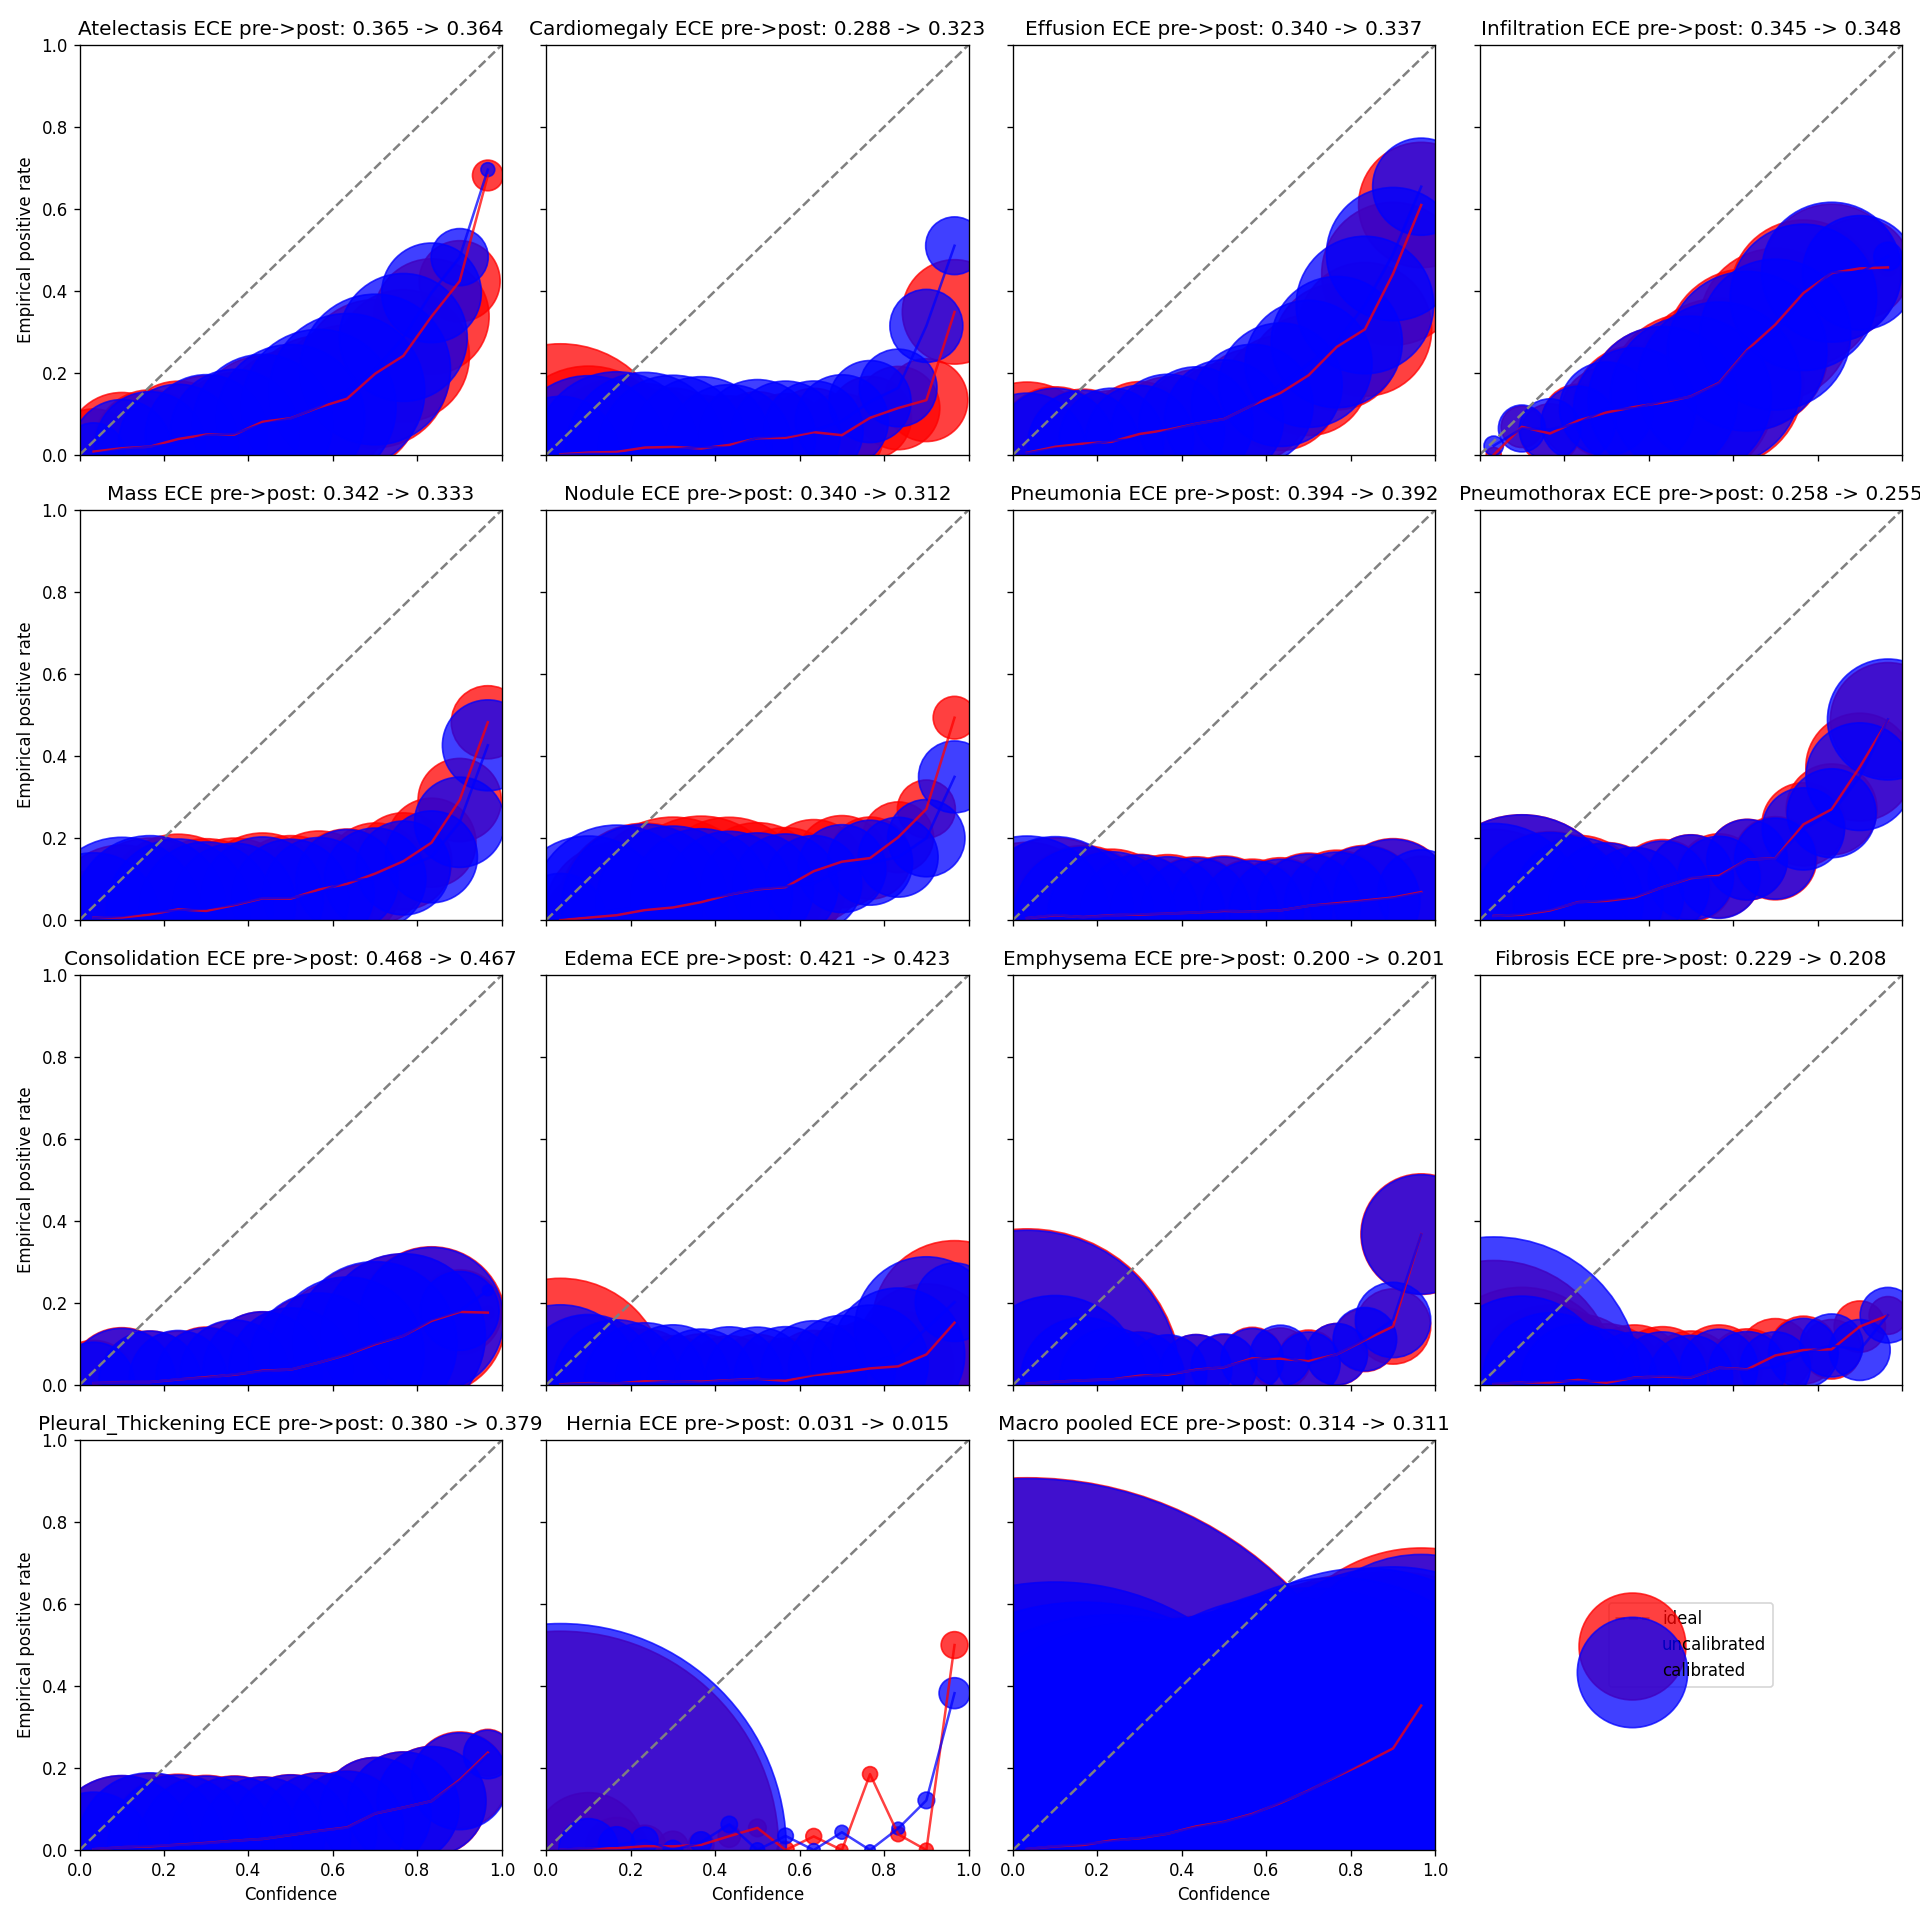
\includegraphics[width=0.8\linewidth]{../results/reliability_diagram.png}
\caption{Reliability diagram generated by \texttt{make calibrate}.}
\end{figure}
}{Calibration figure not found at compile time.}

\subsection{RSNA Overlay Figure}

\IfFileExists{../results/overlays/rsna/rsna_grid.png}{
\begin{figure}[H]
\centering
\includegraphics[width=0.95\linewidth]{../results/overlays/rsna/rsna_grid.png}
\caption{RSNA Pneumonia/Lung Opacity Grad-CAM review grid. This is a weak engineering artifact, not clinical evidence.}
\end{figure}
}{RSNA overlay grid not found at compile time.}

\subsection{CAM Threshold Sweep: Scale vs. Position Error}

The RSNA grounding numbers in the summary table above come from a single operating
point. To understand what drives the near-zero mAP@0.5 despite a pointing-game score
well above chance, \texttt{cam\_threshold} was swept over seven values on the RSNA
\textbf{validation} split (\texttt{results/sweep/}), with CAM boxes extracted per
connected component:

\begin{center}
\begin{tabular}{ccccc}
\toprule
CAM threshold & mAP@0.5 & Mean IoU & IoU $\geq$ 0.5 & Pointing-game \\
\midrule
0.30 & 0.0000 & 0.1388 & 0.0000 & 0.5138 \\
0.40 & 0.0000 & 0.1723 & 0.0000 & 0.5138 \\
0.50 & 0.0001 & 0.2138 & 0.0183 & 0.5138 \\
0.60 & 0.0004 & 0.2570 & 0.0275 & 0.5138 \\
0.70 & 0.0013 & 0.2923 & 0.0550 & 0.5138 \\
\textbf{0.80} & \textbf{0.0045} & \textbf{0.2993} & \textbf{0.1193} & 0.5138 \\
0.90 & 0.0022 & 0.1968 & 0.0550 & 0.5138 \\
\bottomrule
\end{tabular}
\end{center}

Raising the threshold from 0.60 to 0.80 increases mAP@0.5 by a factor of $10.8\times$
(0.00042 to 0.00454) and raises the fraction of boxes reaching IoU $\geq$ 0.5 from 2.8\%
to 11.9\%; the curve is unimodal and falls again at 0.90, so shrinking the box further
is not a fix. Pointing-game accuracy, by contrast, is exactly 0.5138 at every one of the
seven thresholds. This is not a coincidence: pointing-game only checks whether the CAM's
peak activation falls inside the ground-truth box, while thresholding prunes the support
around that peak without moving it. Threshold tuning can therefore correct a scale
error but not a position error, and even at the best threshold 88\% of positives still
fail the IoU $\geq$ 0.5 criterion. This scale/position split, and the resulting gap
between a loose point-based hit rate and a strict IoU-based one, is consistent with the
benchmarked divergence between saliency-metric families reported for chest X-ray
interpretation \citep{saporta2022benchmarking}.

The flatness claim above — pointing-game constant across all seven thresholds — is a
\textbf{validation-split} finding. Threshold and extraction-method selection used only
that split; \texttt{cam\_threshold = 0.80} with \texttt{box\_extraction = multi} was
then read once, as a single confirmatory point, on the held-out RSNA test split (summary
table above): mAP@0.5 0.0091, mean IoU 0.3139, IoU $\geq$ 0.5 hit rate 0.1607, and
pointing-game 0.4286. This single test point does not itself test flatness across
thresholds; only the validation sweep does that. Three of the four localization metrics
are \emph{higher} on this test read than the corresponding validation values at
threshold 0.80 (mAP@0.5 0.0045 $\to$ 0.0091; IoU $\geq$ 0.5 hit rate 0.1193 $\to$
0.1607; mean IoU 0.2993 $\to$ 0.3139); only pointing-game moved the other way (0.5138
$\to$ 0.4286). At $n = 112$ gated positive cases, a proportion near 0.5 has a standard
error of approximately $\sqrt{0.5 \times 0.5 / 112} \approx 0.047$, so the 8.5-point gap
is about $1.8$ standard errors — consistent with sampling noise on a different image
subset rather than a systematic regression. Consistent with not tuning on test,
\texttt{cam\_threshold} and \texttt{box\_extraction} were not revisited in response to
this result.

\subsection{Artifact Audit}

\begin{longtable}{p{0.29\linewidth} p{0.1\linewidth} p{0.2\linewidth} p{0.18\linewidth} p{0.15\linewidth}}
\toprule
Artifact & Exists & Source & Status & Notes \\
\midrule
\endhead
\texttt{checkpoints/baseline\_nih\_best.pt} & local & \texttt{make train} & real & epoch 4 checkpoint, git-ignored \\
\texttt{results/baseline\_nih\_eval.json} & yes & \texttt{make eval} & real & NIH metrics \\
\texttt{results/calibration\_report.json} & yes & \texttt{make calibrate} & real & ECE report \\
\texttt{results/reliability\_diagram.png} & yes & \texttt{make calibrate} & real & reliability figure \\
\texttt{results/grounding\_rsna\_eval.json} & yes & \texttt{make eval-grounding-rsna} & real & pneumonia only \\
\texttt{results/overlays/rsna/rsna\_grid.png} & yes & \texttt{make eval-grounding-rsna} & review artifact & not clinical evidence \\
\texttt{data/vqa/*.jsonl} & local & \texttt{make vqa-dataset} & generated, git-ignored & weak VQA supervision exists locally \\
\texttt{results/vlm\_zero\_shot\_eval.json} & yes & \texttt{make eval-vlm-zero-shot} & partial/blocker & rule-based baseline computed; VLM backend missing \texttt{bitsandbytes} \\
\texttt{results/vlm\_lora\_train.json} & yes & smoke/blocker check & not trained & adapter training implemented; current artifact has zero epochs \\
\bottomrule
\end{longtable}
